% Standalone CSSG schematic — compile: pdflatex causal_state_graph.tex
\documentclass[border=2pt]{standalone}
\usepackage{tikz}
\usetikzlibrary{arrows.meta,positioning}

\begin{document}
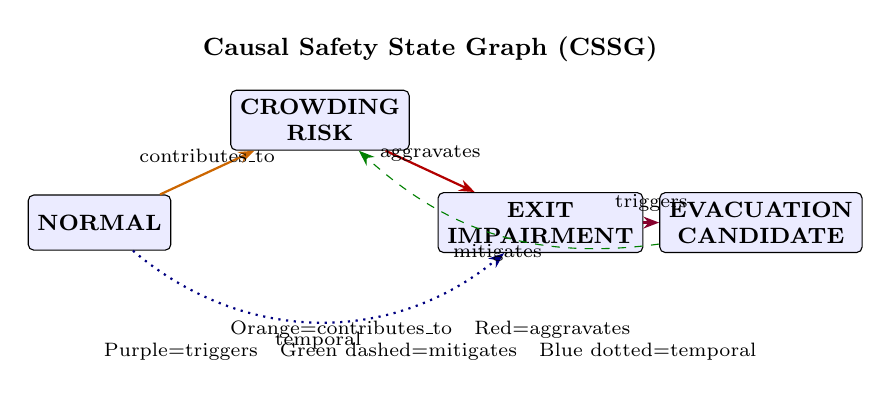
\begin{tikzpicture}[
  state/.style={draw, rounded corners=2pt, minimum width=1.55cm, minimum height=0.7cm,
                align=center, font=\footnotesize\bfseries, fill=blue!8},
  contributes/.style={-{Stealth[length=2mm]}, draw=orange!80!black, thick},
  aggravates/.style={-{Stealth[length=2mm]}, draw=red!70!black, thick},
  triggers/.style={-{Stealth[length=2mm]}, draw=purple!70!black, very thick},
  mitigates/.style={-{Stealth[length=2mm]}, draw=green!50!black, dashed},
  temporal/.style={-{Stealth[length=2mm]}, draw=blue!50!black, thick, dotted},
]

\node[state] (normal) at (0,0) {NORMAL};
\node[state] (crowd) at (2.8,1.3) {CROWDING\\RISK};
\node[state] (exit) at (5.6,0) {EXIT\\IMPAIRMENT};
\node[state] (evac) at (8.4,0) {EVACUATION\\CANDIDATE};

\draw[contributes] (normal) to node[above, font=\scriptsize] {contributes\_to} (crowd);
\draw[aggravates] (crowd) to node[above, font=\scriptsize] {aggravates} (exit);
\draw[triggers] (exit) to node[above, font=\scriptsize] {triggers} (evac);
\draw[temporal] (normal) to[bend right=40] node[below, font=\scriptsize] {temporal} (exit);
\draw[mitigates] (evac) to[bend left=25] node[below, font=\scriptsize] {mitigates} (crowd);

\node[font=\small\bfseries] at (4.2,2.2) {Causal Safety State Graph (CSSG)};
\node[font=\scriptsize, align=center] at (4.2,-1.5) {Orange=contributes\_to\quad Red=aggravates\\
Purple=triggers\quad Green dashed=mitigates\quad Blue dotted=temporal};

\end{tikzpicture}
\end{document}
